\section{Method}
\label{SECII}\label{sec:method}
\subsection{The standard approach: matched filtering}
Compact binary coalescence searches typically employ matched filtering as the
first step to locating a gravitational wave signal ~\cite{findchirppaper}.  
A template waveform is convolved with the whitened data, and if 
properly normalized it produces a signal-to-noise ratio (SNR) that indicates the
probability of a signal being present ~\cite{wainstein:1962}.  
Since the parameters of the signal are
not known apriori, multiple templates must be filtered for a wide range of
parameters.  Let us assume that the waveforms are simply parameterized by
component mass and denote the $i$th template waveform of $N$ templates necessary
to search a given parameter space as $h_i(t) = f(m1,m2,t)$.
The SNR, $\rho_i$ for that template is
\begin{equation}
\label{eq:time_domain_snr}
\rho_i(t) = \int h_i(t) s(t-\tau) \, d\tau,
\end{equation}
where $s(t)$ is the detector data stream suitably whitened having mean zero
and unity variance.  Time domain convolutions don't have any inherent latency. 
The template waveform can be ``slid onto" the detector data as it is produced
giving the possibility of measuring a peak SNR at the time of inspiral
coalescence.  Typically it is not tractable to compute SNR via a
time domain convolution as indicated in (\ref{eq:time_domain_snr}) because
it involves an $\mathcal{O}(N^2)$ operation per template. Instead the
convolution theorem is applied and the SNR is obtained via an inverse Fourier
transform
\begin{equation}
\label{eq:freq_domain_snr}
\rho_i(t) = \int \tilde{h}_i(f)\,^*\,\tilde{s}(f)\,e^{-2\pi i f t}\, df,
\end{equation}
where the $\tilde{h}_i(f)$ and $\tilde{s}(f)$ denote the Fourier transforms
of the template and detector data respectively.  This operation is far
faster to compute with $\mathcal{O}(N\,{\rm log}\,N)$ operations per template.  
However, the acausal nature of the Fourier transform introduces an inherent
latency.  One must wait until they have collected data as long as their 
signal and for minimally overlapping computations that means having a latency
about as long as the template waveform.  The latency can be reduced by having
redudant overlapping transforms, but at an additional cost.  

Thus we have that low latency searches are inherently more computationally
costly than moderate latency searches that employ frequency domain matched
filtering.  The next section discusses a method to mitigate the cost of
low latency searches. 

\subsection{Reducing the number of filters with singular value decomposition}
It is clear that in order to reduce the cost of a low latency search for
compact binaries of unknown mass we need to reduce the number of convolutions
necessary to find the gravitational-wave signal.  Rather than filter the
$i$ templates corresponding to binaries of different component masses it is
possible to find a basis set of fewer filter $u_j$ that can be linearly combined
to reproduce $\rho_i$ to some accuracy.  For the remainder of this section
we will drop the explicit time dependence of the convolution and recognize
that the snr for any point in time is simply the innerproduct between a
template waveform vector ${\bf \hat{h}_i}$ and a vector of the detector data 
${\bf \hat{s}}$, $\rho_i = ({\bf \hat{h}_i}|{\bf \hat{s}})$.  
The goal is to have
\begin{equation}
\label{eq:linear_combination_of_snr}
\rho_i = \sum_{j=1}^{N'} M_{ij} ({\bf \hat{u}_j}|{\bf \hat{s}})
\end{equation}
where the number of inner products is reduced from $N$ to $N'$. In order to
find the basis set ${\bf u_j}$ we use the singular value decomposition of
the matrix 
${H_{ik}} = \{{\bf \hat{h}_1}, {\bf \hat{h}_2}, ...{\bf \hat{h}_N}\}$. Where
$i$ is the index over the template number and $k$ is the index over sample 
points. The singular value decomposition factors a matrix such that
\begin{equation}
\label{eq:svd}
{H_{ik}} = {A_{ij}\,B_{jl}\,U_{lk}}
\end{equation}
The matrix ${B_{jl}}$ is a diagonal matrix of singular values ranked in
order of importance of reconstructing the original matrix ${H_{ik}}$.
However since a search for binary inspirals only needs  waveform accuracy to a
few percent to be successful it is possible to make an approximate 
reconstruction of ${H_{ik}}$ 
\begin{equation}
\label{eq:svdapprox}
{H_{ik}} \approx {A_{ij}\,B'_{jl}\,U_{lk}}
\end{equation}
where the rank of ${B'_{jl}}$ is less than the rank of ${B_{jl}}$.
This reduces the number of rows in ${U_{lk}}$.  Now we have a 
new basis of template waveforms derived from ${U_{lk}} = \{{\bf \hat{u}_1}, {\bf \hat{u}_2}, ...{\bf \hat{u}_{N'}}\}$ and can write 
(\ref{eq:linear_combination_of_snr})
\begin{eqnarray}
\label{eq:svdsnr}
\rho_i &=& \sum_{j=1}^{N'} A_{il}\,B'_{lj} ({\bf \hat{u}_j}|{\bf \hat{s}}) \nonumber \\
       &=& \sum_{j=1}^{N'} M_{ij} ({\bf \hat{u}_j}|{\bf \hat{s}})
\end{eqnarray}

This result differs from other work that models gravitational-wave chirp
signals in approximate ways 
~\cite{Chassande-Mottin2006, Candes2008, BuonannoChenVallisneri:2003a} 
by starting with an exact representation of the desired template family and
producing a rigorous approximation with a tunable accuracy.  

\subsection{Detection statistic}
It is not necessary to reconstruct the SNR of all templates in order to 
determine if a signal is present.  By thresholding on the sum of squares
of the orthoganal decomposition described above it is possible to answer
whether or not an inspiral like event is in the data.  Then only 
potentially interesting times can be reconstructed on a sample by sample 
basis.  Following the ideas in ~\cite{Anderson:2000yy} we employ a detection
statistic as
\begin{equation}
\label{eq:stat}
\Gamma^2 = \sum_{l} \sum_{j} {B'_{lj}}^2 {({\bf \hat{u}_j}|{\bf \hat{s}})}^2
\end{equation}


\subsection{Signal consistency check}
After reconstructing the SNR of an individual template it is possible to 
to check that the components along the SVD basis were consistent with 
expectation by performing a $\chi^2$ fit to the decomposition.  
\begin{equation}
\label{eq:chisq}
\chi^2_i = \sum_j {[({\bf \hat{u}_j}|{\bf \hat{s}}) - \rho_i / M_{ij}]}^2
\end{equation}


\subsection{Selectively reducing the sample rate of the data and template
waveforms}
The computational cost of filtering can be further reduced by selectively
downsampling certain intervals of the template waveform.  Note that the
frequency of gravitational radiation resulting from the inspiral of two
compact object is given by the quadrupole aproximation as ~\cite{finn1993}
\begin{equation}
\label{eq:fgw}
f_{\rm GW} = \frac{1}{\mathcal{\pi M}} \left[ \frac{5}{256}\frac{\mathcal{M}}{t_c} \right]^{3/8}
\end{equation}
where $\mathcal{M}$ is the chirpmass in units of $G=c=1$ and $t_c$ is the time
before the coalescence of the binary.  Typically the filter is integrated to
a finite frequency, $f_e$ which corresponds to a time, $t_e$ before the 
coalescence~\cite{kidder1992, blanchet2002, findchirppaper, hanna2009}.  Given
the relationship $f/f_e = (t_e/t)^{3/8}$ it is possible to reduce a
filter waveform into critically sampled bands by dividing them up in time.
This is possible regardless of the time-frequency relationship as long as
it can be computed rigorously and thus the method doesn't depend on 
(\ref{eq:fgw}).  As a concrete example consider a waveform obeying 
(\ref{eq:fgw}) with a chirp mass of 1 $M_{\odot}$ for which we decide
to cut the filter at $f_e = 2048$Hz (corresponding to $t_e = 0.00093$s).  
It is then possible to compute sub bands which are each critically sampled
according to table \ref{table1}  
\begin{table}[!h]
\caption{
Example critically sampled sub bands for a 1 $M_{\odot}$ filter with a 
time frequency structure given by ($\ref{eq:fgw})$.  Most of the filter is
low frequency and it is possible to save computation by breaking up the filter
into bands each of which has restricted frequency content. 
}
\begin{center}
\label{table1}
\begin{tabular}{@{} lll @{}}
\hline
\hline
Sub band & Sample rate (Hz) &Interval (s) \\
\hline
1 & 2048 & [0.00093, 0.0059] \\
2 & 1024 & [0.0059, 0.037]  \\
3 & 512  & [0.037, 0.24]   \\
4 & 256  & [0.24, 1.51]   \\
5 & 128  & [1.51, 9.60]   \\
6 & 64   & [9.60, 60.95]  \\
7 & 32   & [60.95, 387.0]  \\
\hline
\end{tabular}
\end{center}
\end{table}
where it is assumed that the filter is cut to some finite length, 387s 
for this example.  This idea has been demonstrated by the Virgo Collaborations
MBTA pipeline~\cite{beauville2006, beauville2008}.

\subsection{Comparison of computational costs and latency}
Convolutions are best done with the use of the Fast Fourier Transform (FFT).
However there is an inherent latency in performing convolutions this way. This
section describes the computational cost and latency of FFT convolutions, time 
domain (TD) convolutions and TD convolutions with SVD.  

Convolving one filter with data using FFTs involves 
$\mathcal{O}[10 N_s \log_2(N_s)]$
floating point operations where $N_s$ is the number of sample points in
the data being convolved and results in $N_s - N_f$ samples of usable output.  
In comparison time domain convolutions require
$\mathcal{O}[N_s N_f]$ where $N_f$ is the number of sample points in the
filter.  The FFT is faster to compute when $N_f > 10 \log_2(N_s)$.  However
the FFT has an inherent latency of $\mathcal{O}[N_s/f_s]$ seconds, where
$f_s$ is the sample rate when minimally overlapping FFTs are computed. It is
possible to reduce the latency of the FFT by performing vastly overlapping
FFTs.  The cost of such a procedure would be 
$\mathcal{O}[10 N_o N_s \log_2(N_s)]$.  Thus for comparable computational
cost where $N_f \approx 10 N_o \log_2(N_s)$ the latency of the FFT method 
would be $\mathcal{O}[N_s/f_s/N_o]$ seconds.  Depending on the task at hand,
latency requirements and computational costs can dictate what procedure to
use.  

\subsection{Data Whitening}
Matched filtering the SVD basis vectors has motivated a decoupling of the
whitening routine from the matched filtering engine. This was necessary in
order weight templates appropriately by whitening them before the SVD
calculation, and, as such, we have also moved the data whitening outside the
match filter engine. We have chosen to whiten the data using a running
geometric average of the PSD computed by Hann windowing 8 second buffers of
data and using 50\% overlapping buffers. The running geometric average is
updated once per buffer from a median of the recent PSDs. We find that this
algorithm is extremely fast to converge to an accurate PSD and also very robust
against glitches. This is demonstrated below where we have injected
band-limited white noise burst with a central frequency of 150 Hz, a bandwidth
of 100 Hz, a time duration of 0.2 seconds, and a injection density of one
injection every $100/\pi \approx 32$ seconds. At this density we find there
should only ever be one injection affecting the median history so the glitches
should minimally affect PSD estimation as can be seen by comparing the local
RMS amplitude between injections to that without injections.

\begin{center}
\resizebox{0.9\textwidth}{!}{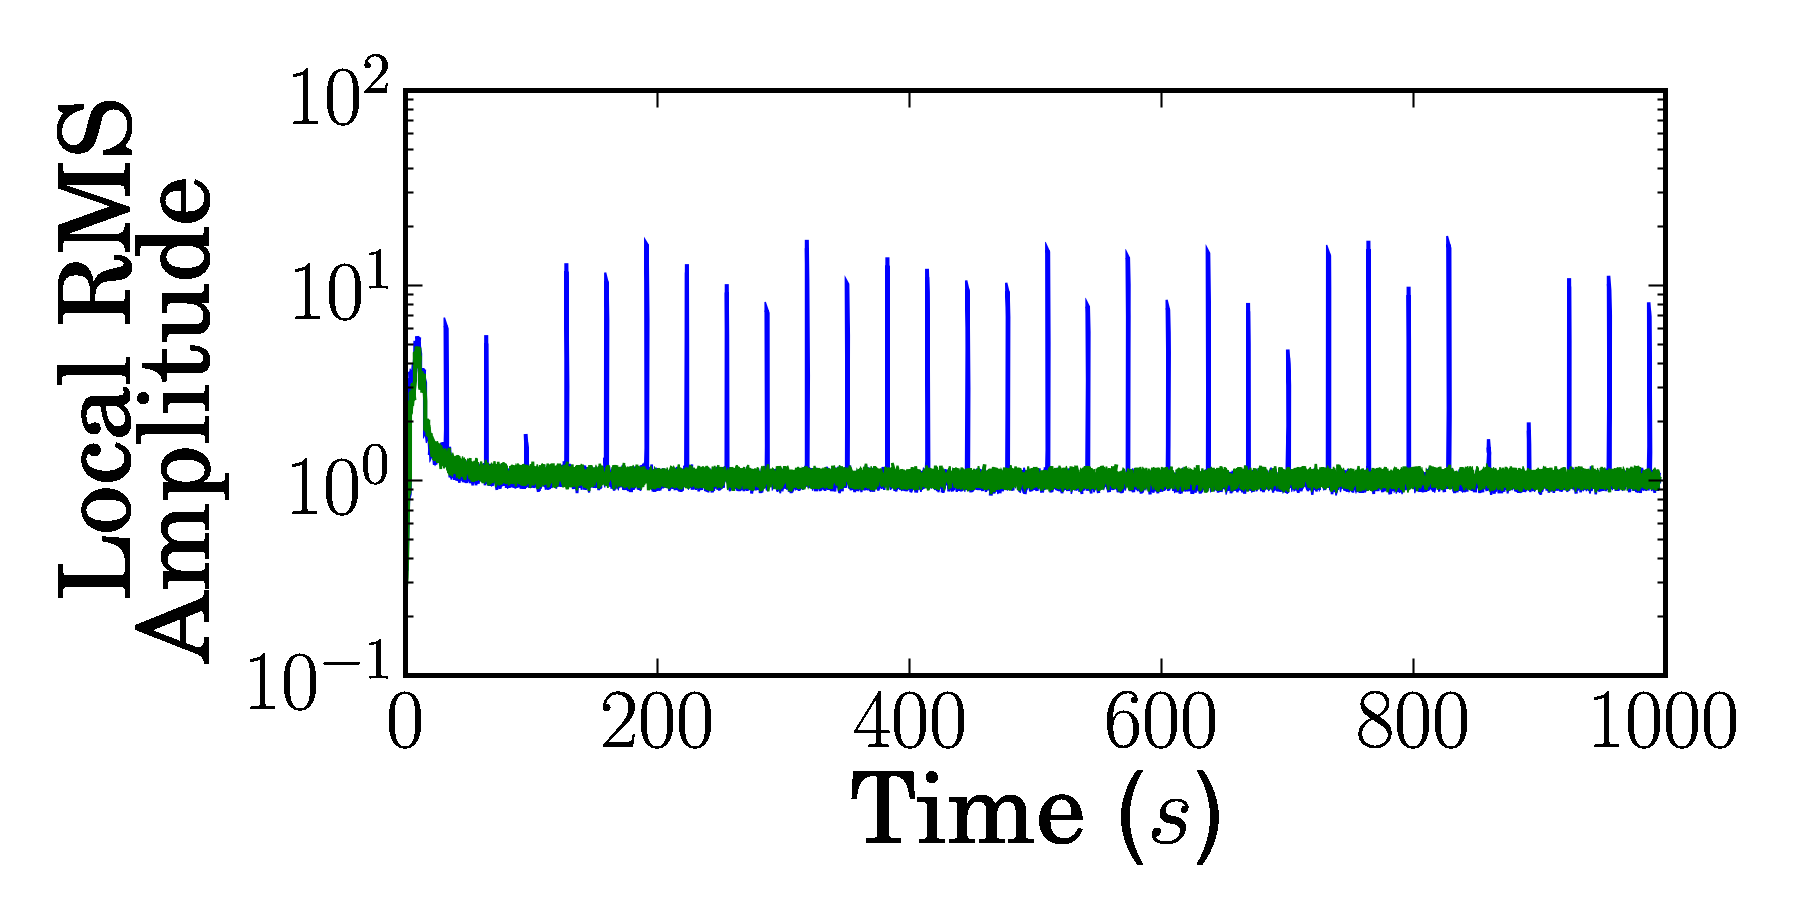
\includegraphics{figures/whiten_burst_step_100_semilogy.png}}
\end{center}

An inspiral, to leading order, has gravitational-wave frequency evolution given
by
\begin{equation}
f(t) = \frac{1}{8 \pi \mathcal{M}} \left( \frac{t_c - t}{5 \mathcal{M}} \right)^{-3/8}\;,
\end{equation}
whose time derivative is given by
\begin{equation}
\frac{df}{dt} = \frac{3}{320 \pi \mathcal{M}^2} \left( \frac{t_c - t}{5 \mathcal{M}} \right)^{-11/8}\;.
\end{equation}
Combining these, we find the frequency evolution as a function of frequency to
be
\begin{equation}
\frac{df}{dt}(f_0) = \frac{3}{320 \pi \mathcal{M}^2} \left( 8 \pi \mathcal{M} f_0 \right)^{3/11}\;,
\end{equation}
which can be inverted to get the minimum frequency which has a given frequency
derivative,
\begin{equation}
f_0 = \frac{1}{8 \pi \mathcal{M}} \left( \frac{320 \pi \mathcal{M}^2}{3} \frac{df}{dt} \right)^{11/3}\;.
\end{equation}

If we allow frequency bins to be affected by an injection only once within the
median history, we need to calculate the corresponding $df/dt$ for our PSD
calculation. An FFT of a buffer with length $T$ will have a frequency
resolution $df = 1/(2T)$. Hann windowing the data and overlapping buffers by
50\% introduces correlations in neighboring frequency bins of the FFT. This
means that we actually want the frequency to change by $df = 3/(2T)$ before the
next PSD calculation, which happens a $dt = T/2$ later, resulting in a minimum
$df/dt = 3/T^2$.

Combining these results we find the lower frequency bound for our injections,
assuming a chirp mass for a binary with $m_1 = m_2 = 1 M_{\odot}$ and $T = 8$
s, is 23 Hz.

We want to compute the equivalent injection density which would be biased as
much as lalapps\_inspiral's PSD estimator, which allows $\sim3$ injections per
2048 seconds. It computes the PSD by breaking the segment up into 16 256 second
chunks. These chunks are then combined into to sets of 8 chunks each. The
median of each set is then averaged across the sets for each frequency bin to
produce the PSD estimate for that 2048 second segment. This procedure results
in an average injection density of 1.5 per 8 PSDs in the median history, which
is comparable to LLOID's 1 per 7 PSDs in the median history. Since LLOID has an
injection history of 7 PSDs which span 32 seconds, this means LLOID can perform
one injection every 32 seconds, or 64 injections per 2048 second segment, more
than an order of magnitude increase in density over lalapps\_inspiral.


